\section{Graph Interconnection, Rotor Energy, and Bayesian Evidence}
\label{app:hamiltonian-graph}
\newcommand{\HamWorkError}{1.06\times10^{-2}}
\newcommand{\HamTorqueError}{1.01\times10^{-15}}
\newcommand{\HamNetworkError}{4.13\times10^{-11}}
\newcommand{\HamPredictionError}{1.53\times10^{-14}}
\newcommand{\HamLoglikError}{1.91\times10^{-6}}

The graph enters through electrical operators. The plant has 114
differential states, including ten Sauer--Pai machines and controls;
its augmented predictor has 376 coordinates. Rotor angle $\delta_g$,
per-unit absolute speed $\omega_g$ and the deviation vector $\Delta x$
are distinct. PMU frequency comes from voltage phase, not rotor speed.

\begin{figure*}[t]\centering
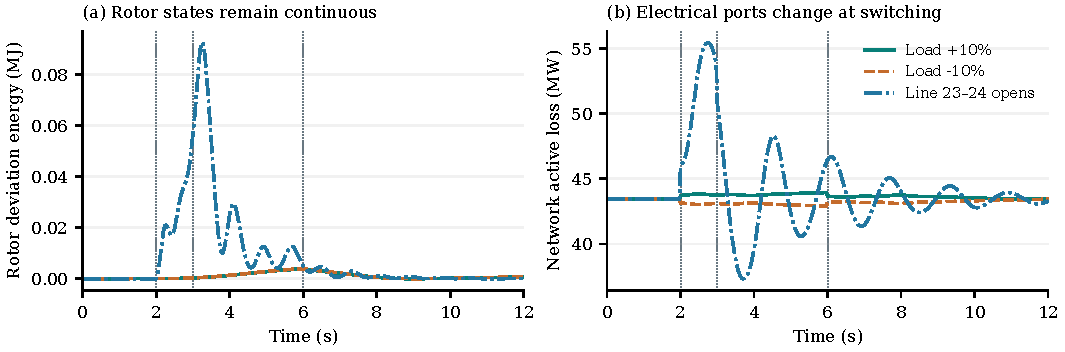
\includegraphics[width=.96\textwidth]{figures/generated/hamiltonian_balance.pdf}
\caption{New nonlinear IEEE-39 consistency trajectories. Changes begin at
2\,s; the line is restored at 3\,s and loads at 6\,s. The normal trajectory
has zero rotor deviation energy and is omitted for clarity. Rotor energy
uses simulated internal states, not eight-PMU measurements. The traces
verify the mechanical/electrical connection; they do not establish an
energy-based event detector.}
\label{fig:hamiltonian-balance}
\end{figure*}

\subsection{An Exact Mechanical Subsystem Balance}
The implemented machine equations, with frame speed one, are
\begin{align}
 \dot\delta_g&=\omega_b(\omega_g-1),\nonumber\\
 2H_g\dot\omega_g&=\tau_{m,g}-\tau_{e,g}-D_g(\omega_g-1).
 \label{eq:rotor-torque}
\end{align}
Here $\tau_{m,g},\tau_{e,g}$ are per-unit torques on machine rating $S_g$;
$\omega_b$ is in rad/s and $H_g$ in seconds. Multiplying the second
equation by $S_g\omega_g$ gives the exact kinetic balance
\begin{align}
 K&=\sum_g S_gH_g\omega_g^2,\nonumber\\
 \dot K&=\sum_g S_g\omega_g
 [\tau_{m,g}-\tau_{e,g}-D_g(\omega_g-1)].
 \label{eq:kinetic-port-balance}
\end{align}
With ratings expressed numerically in MVA on the model's power bases,
$K$ is in MJ and its derivative in MW. The algebraic stator equations
also imply, on each machine base,
\begin{equation}
 \omega_g\tau_{e,g}=P_g+R_{s,g}(I_{d,g}^2+I_{q,g}^2).
\end{equation}
Replacing torque by terminal power without this speed factor would change
the implemented dynamics. Governor torque and electromagnetic torque
remain ports of this mechanical subsystem; their evolution is not discarded.

A canonical description of the rotor deviations follows by defining
\begin{align}
 p_g&=\frac{2H_gS_g}{\omega_b}(\omega_g-1),\nonumber\\
 \mathcal H_{\rm rot}(p)&=\sum_g\frac{\omega_b^2p_g^2}{4H_gS_g}.
\end{align}
Then $\dot\delta_g=\partial\mathcal H_{\rm rot}/\partial p_g$ and
\begin{equation}
 \dot p_g=\frac{S_g}{\omega_b}(\tau_{m,g}-\tau_{e,g})
 -\frac{S_gD_g}{\omega_b^2}\frac{\partial\mathcal H_{\rm rot}}{\partial p_g}.
\end{equation}
This is a Hamiltonian rotor subsystem with torque ports and nonnegative
damping when $D_g\ge0$. In this fixed plant direct shaft damping is zero;
controller dynamics are still present. Neither $K$ nor
$\mathcal H_{\rm rot}$ is a total energy or a Lyapunov function for the
complete lossy DAE. A global port-Hamiltonian realization would require
compatible electrical storage and controller interconnections
\cite{fiaz2013port}.

\subsection{The Graph Connects Electrical Power Ports}
Let $C_f,C_t$ select the source and destination buses of each branch,
including the declared transformer orientation. With outward terminal
currents,
\begin{align}
 i_f&=Y_{f,q}V,\quad i_t=Y_{t,q}V,\nonumber\\
 i_{\rm net}&=C_f^\top i_f+C_t^\top i_t.
\end{align}
The branch and nodal active powers obey the algebraic identity
\begin{equation}
 \Re(V^\top\overline{i_{\rm net}})=
 \Re[(C_fV)^\top\overline{i_f}+(C_tV)^\top\overline{i_t}].
 \label{eq:graph-power-ports}
\end{equation}
Separately modeled bus shunts must be added if present. The actual branch
stamps retain resistance, charging and transformer ratios; a simple
lossless Laplacian is insufficient. Opening a branch changes these ports
and the algebraic solution while differential states, hence rotor energy,
remain continuous. The ports affect electrical torque, which then changes
rotor motion. This connects graph structure to recovery without introducing
an independent energy observation.

\subsection{Executed Physical and Inference Controls}
Four new 12-s trajectories use the unmodified nonlinear plant and initial
condition: normal, a $+10\%$ and a $-10\%$ change of the bus-7 impedance
load's P/Q setpoints from 2 to 6\,s, and opening line 23--24 from 2 to 3\,s.
Actual load power remains voltage-dependent. All four solves succeed,
with zero detected differential-state jump. At 120 samples/s the largest
rotor-equation residual is $\HamTorqueError{}$ and the largest
generation--load--network-loss mismatch is $\HamNetworkError{}$ system pu.
Numerically integrating mechanical work separately on smooth segments
gives maximum kinetic-energy discrepancy $\HamWorkError{}$ MJ; intervals
ending at a switching instant are excluded from trapezoidal integration.
These are physical consistency checks, not independent statistical
replicates or event-detection results.



To test whether the energy coordinates themselves add inferential value,
let $\eta=L\xi$ be their invertible linear scaling of deviation coordinates.
Every operator must be transformed consistently:
\begin{align}
 T'_q&=LT_qL^{-1},&J'_q&=J_qL^{-1},\nonumber\\
 g'_q&=Lg_q,&u'_q&=Lu_q,\nonumber\\
 P'_h&=LP_hL^\top,&K'_h&=LK_h.
\end{align}
Transform means, severity directions and process covariance likewise;
observation offsets and noise stay unchanged. Predicted reports and
innovation distributions then coincide. Transforming the state prior
with its Jacobian also preserves the integrated likelihood. Thus an
exact Bayesian comparison with the same histories and publication rules
gains no information. Coordinate-dependent approximations need a separate check.

Using all 18 nominal source operators through ON, stay and OFF, the maximum
relative prediction discrepancy is $\HamPredictionError{}$. In 180 paired
Gaussian known-signature draws, native and rotor-coordinate likelihoods
select the same source every time. The largest absolute log-likelihood
discrepancy, $\HamLoglikError{}$, exceeds the preset $10^{-6}$ numerical
gate; this gate remains failed. The result is reported as a finite-precision
limitation, not as an all-checks-pass certification. This control does not
rerun the bank's proposal search, pruning or unknown-severity integration.
It supplies no evidence of improved attribution.

Energy reconstructed from the same PMUs is not independent evidence.
An energetic prior or discrepancy constraint would change the model and
require a new comparison. The validated result is a mechanical interpretation
and its graph coupling; no additional event score or accuracy gain is established.
